%%%%%%%%%%%%%%%%%%%%%%%%%%%%%%%%%%%%%%%%%%%%%%%%
%% Compile the master file!
%% 		Slides: Antonio Machicao y Priemer
%% 		Course: Wissenschaftliches Arbeiten
%%%%%%%%%%%%%%%%%%%%%%%%%%%%%%%%%%%%%%%%%%%%%%%%


%%%%%%%%%%%%%%%%%%%%%%%%%%%%%%%%%%%%%%%%%%%%%%%%%%%%
%%%             Metadata                         
%%%%%%%%%%%%%%%%%%%%%%%%%%%%%%%%%%%%%%%%%%%%%%%%%%%%  

\title{
	\LaTeX\ for Linguists
}

\subtitle{\LaTeX\ 1: Basics}

\author[aMyP]{
	{\small Sebastian Nordhoff \& Antonio Machicao y Priemer}
	\\
	{\footnotesize \url{www.linguistik.hu-berlin.de/staff/amyp}}
	%	\\
	%	{\footnotesize \href{mailto:mapriema@hu-berlin.de}{mapriema@hu-berlin.de}}
}

\institute{LOT 2019, Amsterdam}

%\date{ }

%\publishers{\textbf{6. linguistischer Methodenworkshop \\ Humboldt-Universität zu Berlin}}

%\hyphenation{nobreak}


%%%%%%%%%%%%%%%%%%%%%%%%%%%%%%%%%%%%%%%%%%%%%%%%%%%%
%%%             Preamble's End                   
%%%%%%%%%%%%%%%%%%%%%%%%%%%%%%%%%%%%%%%%%%%%%%%%%%%%      


%%%%%%%%%%%%%%%%%%%%%%%%%%%%%%%%%%%
%%%%%%%%%%%%%%%%%%%%%%%%%%%%%%%%%%%    
%% Title slide 
\begin{frame}
  \HUtitle
\end{frame}


%% Contents slide
\frame{
\begin{multicols}{2}
	\frametitle{Contents}
%	\tableofcontents[hideallsubsections]
	\tableofcontents
	%[pausesections]
\end{multicols}
	}


%%%%%%%%%%%%%%%%%%%%%%%%%%%%%%%%%%%%
%%%%%%%%%%%%%%%%%%%%%%%%%%%%%%%%%%%%
%% Extra literature

\nocite{Freitag&MyP15a}
\nocite{Knuth1986}
\nocite{Kopka94a}
%\nocite{MyP17c}
\nocite{MyP&Kerkhof16a}
	
%%%%%%%%%%%%%%%%%%%%%%%%%%%%%%%%%%%%
%%%%%%%%%%%%%%%%%%%%%%%%%%%%%%%%%%%%


%%%%%%%%%%%%%%%%%%%%%%%%%%%%%%%%%%%%%
%%%%%%%%%%%%%%%%%%%%%%%%%%%%%%%%%%%%%
%%%% Basic literature for these slides
%
%\begin{frame}
%\frametitle{Grundlage \& empfohlene Lektüre}
%
%\dots basierend auf \citet{Freitag&MyP15a} und auf \citet{MyP&Kerkhof16a}\\
%\ras \href{https://www.researchgate.net/publication/279514740_LATEX-Einfuhrung_fur_Linguisten}{LINK}
%
%
%\nocite{Kopka94a}
%
%\end{frame}


%%%%%%%%%%%%%%%%%%%%%%%%%%%%%%%%%%
%%%%%%%%%%%%%%%%%%%%%%%%%%%%%%%%%%
\section{What is \LaTeX ?}
\frame{
%\frametitle{~}
\begin{multicols}{2}
	\tableofcontents[currentsection,hideallsubsections]
\end{multicols}
}
%%%%%%%%%%%%%%%%%%%%%%%%%%%%%%%%%%

\subsection{History}

\begin{frame}
\frametitle{History}

\begin{itemize}
	\item $\tau \epsilon \chi$ (\TeX ) was developed between 1977 and 1986 by Donald E. Knuth.
	
	\item \LaTeX\ is an interface with helpful macros for the \TeX\ system. It was written by Leslie Lamport ($=$ \textbf{La}mport \textbf{\TeX }). 
	
%	\item Pronunciation: \textipa{["la:.tE\c{c}]}, \textipa{["leI.tE\c{c}]}, \textipa{["leI.tEkh]}
	
	\item \LaTeX\ works with markup tagging conventions -- similar to HTML -- to 
	
	\begin{itemize}
		\item define the structure of the document (\fe chapters and sections),
		
		\item for typographic marking (\fe bold and italics), 
		
		\item for cross-references (\fe citations)
	\end{itemize}

\end{itemize}

\end{frame}


%%%%%%%%%%%%%%%%%%%%%%%%%%%%%%%%%%
%%%%%%%%%%%%%%%%%%%%%%%%%%%%%%%%%%
\subsection{WYSIWYG vs. WYGIWYN}
%\frame{
%	%\frametitle{~}
%	\begin{multicols}{2}
%		\tableofcontents[currentsection,hideallsubsections]
%	\end{multicols}
%}

%%%%%%%%%%%%%%%%%%%%%%%%%%%%%%%%%%
\begin{frame}
\frametitle{WYSIWYG vs. WYGIWYN}

\begin{itemize}
	\item \emph{MS Word} or \emph{Libre Office}:
	\textbf{WYSIWYG} (\emph{what-you-see-is-what-you-get}) 
	
	\begin{figure}
		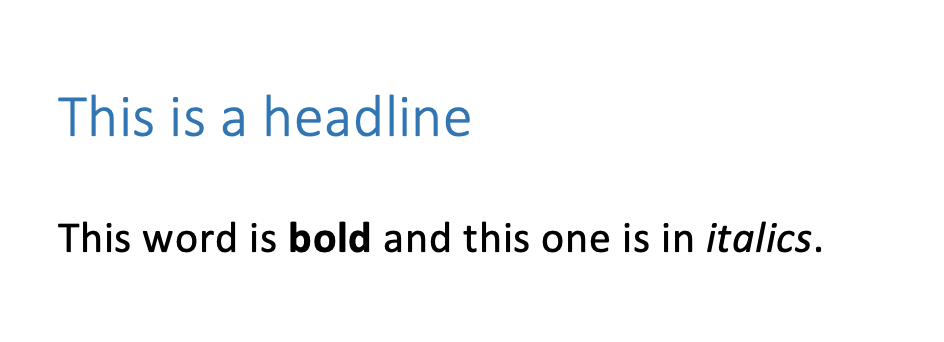
\includegraphics[scale=.3]{../../texfiles-beamer/tex-material/WissArb-latex/WYSIWYG}
	\end{figure}
		
	\item \LaTeX : \textbf{WYGIWYN} or \textbf{WYGIWYM} (\emph{what-you-get-is-what-you-need}/\emph{mean})
	
	\begin{figure}
		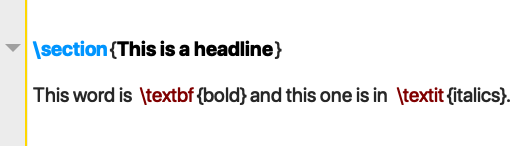
\includegraphics[scale=.3]{../../texfiles-beamer/tex-material/WissArb-latex/WYSIWYM}
	\end{figure}
	
\end{itemize}\end{frame}


%%%%%%%%%%%%%%%%%%%%%%%%%%%%%%%%%%%
%%%%%%%%%%%%%%%%%%%%%%%%%%%%%%%%%%%
%\subsection{Warum sollte ich es benutzen?}
%%\frame{
%%	%\frametitle{~}
%%	\begin{multicols}{2}
%%		\tableofcontents[currentsection,hideallsubsections]
%%	\end{multicols}
%%}
%%
%%%%%%%%%%%%%%%%%%%%%%%%%%%%%%%%%%%
%
%\begin{frame}
%\frametitle{Warum sollte ich es benutzen?}
%
%\begin{itemize}
%	\item Zeitersparnis ({\tiny nicht am Anfang!})
%	\item[]
%
%\pause	
%
%	\item Man hört auf, Sachen zu tun, die der Computer für einen erledigen kann. Daher hat man mehr Zeit, um sich mit dem Inhalt zu befassen.
%	\item[]
%
%\pause	
%
%	\item Die Texte werden sehr gut gesetzt!
%	\item[]
%
%\pause
%
%	\item Ein Programm für alle Funktionen: Artikel, Bücher, Poster, Präsentationen, \dots 
%	\item[]
%
%\pause
%
%	\item Gratis!!
%
%\end{itemize}
%
%\end{frame}


%%%%%%%%%%%%%%%%%%%%%%%%%%%%%%%%%%%
%%%%%%%%%%%%%%%%%%%%%%%%%%%%%%%%%%%
\iftoggle{handout}{
	
%%%%%%%%%%%%%%%%%%%%%%%%%%%%%%%%%%%

%%%%%%%%%%%%%%%%%%%%%%%%%%%%%%%%%%
%%%%%%%%%%%%%%%%%%%%%%%%%%%%%%%%%%
\subsection{Examples}
%\frame{
%	%\frametitle{~}
%	\begin{multicols}{2}
%		\tableofcontents[currentsection,hideallsubsections]
%	\end{multicols}
%}
%%%%%%%%%%%%%%%%%%%%%%%%%%%%%%%%%%%

\begin{frame}
\frametitle{Examples}

What can you do with \LaTeX ?

\end{frame}


%%%%%%%%%%%%%%%%%%%%%%%%%%%%%%%%%%%%
\begin{frame}
\frametitle{Books \& Articles}

%\begin{figure}[htbp]

\begin{minipage}[c]{0.49\textwidth}
\centering
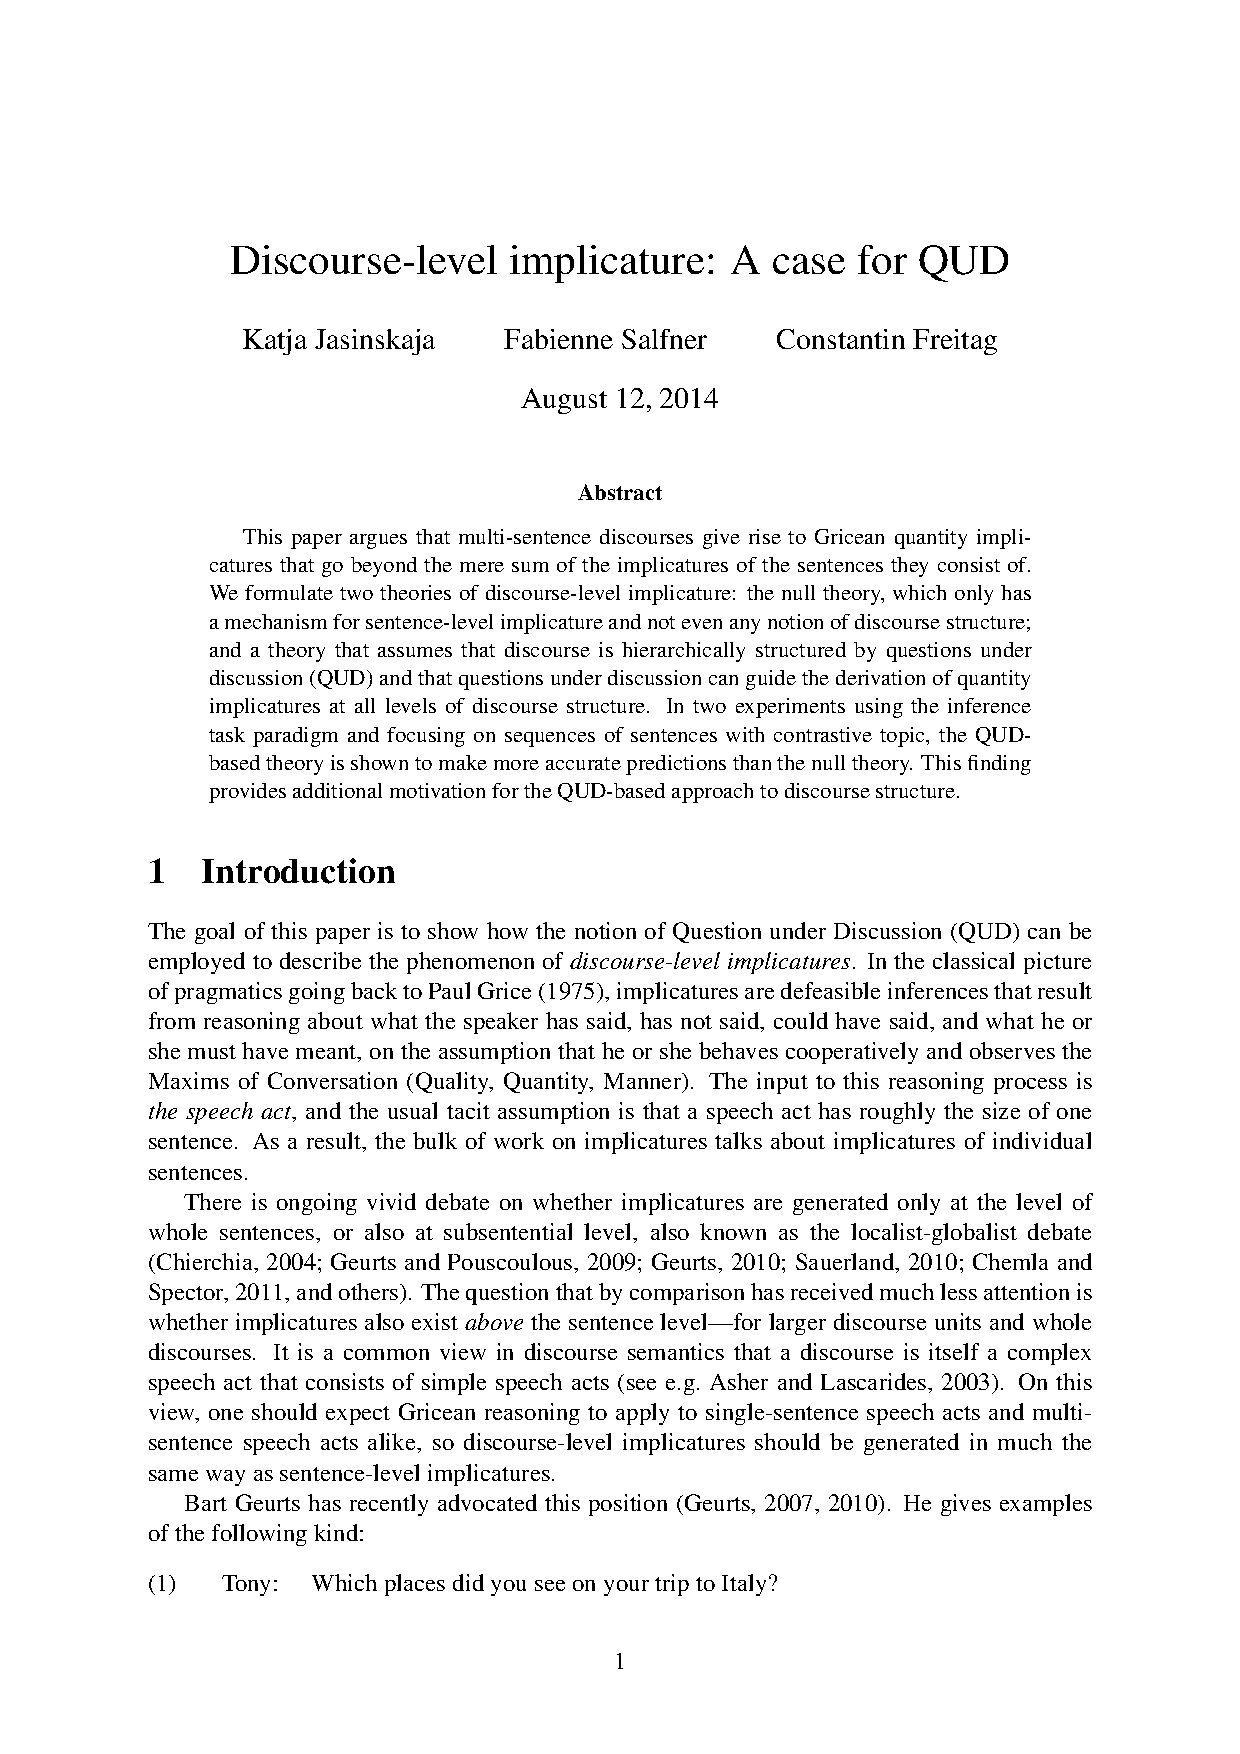
\includegraphics[width=0.80\linewidth]{../../texfiles-beamer/tex-material/WissArb-latex/LaTeX_article.pdf}
\end{minipage}  
%  
\begin{minipage}[c]{0.49\textwidth}
\centering
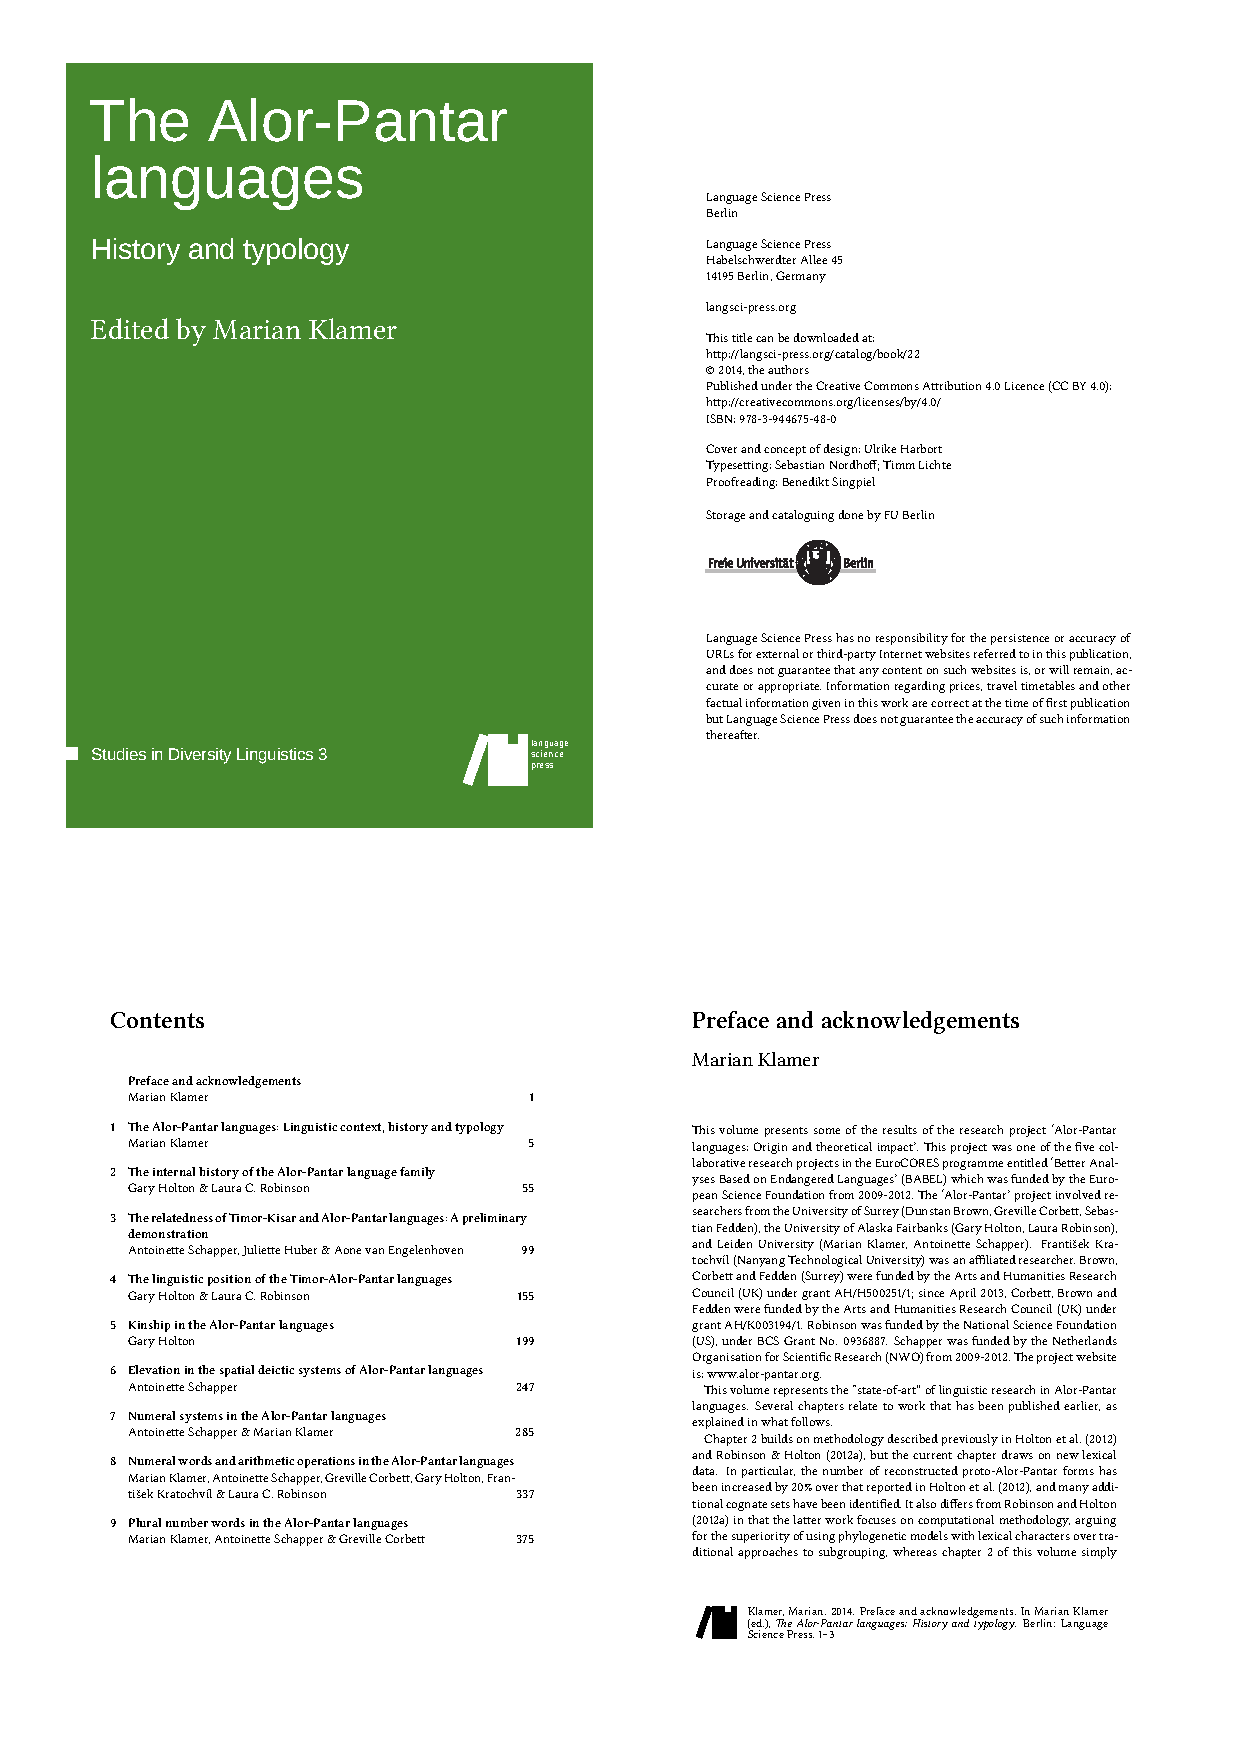
\includegraphics[width=0.80\linewidth]{../../texfiles-beamer/tex-material/WissArb-latex/LaTeX_book_2.pdf}
%\caption{Adjunkt und Komplement}	
\end{minipage}
%         
%\end{figure}

\end{frame}


%%%%%%%%%%%%%%%%%%%%%%%%%%%%%%%%%%%%
\begin{frame}
\frametitle{Poster \& Letter}

%\begin{figure}[b]

\begin{minipage}[b]{0.49\textwidth}
\centering
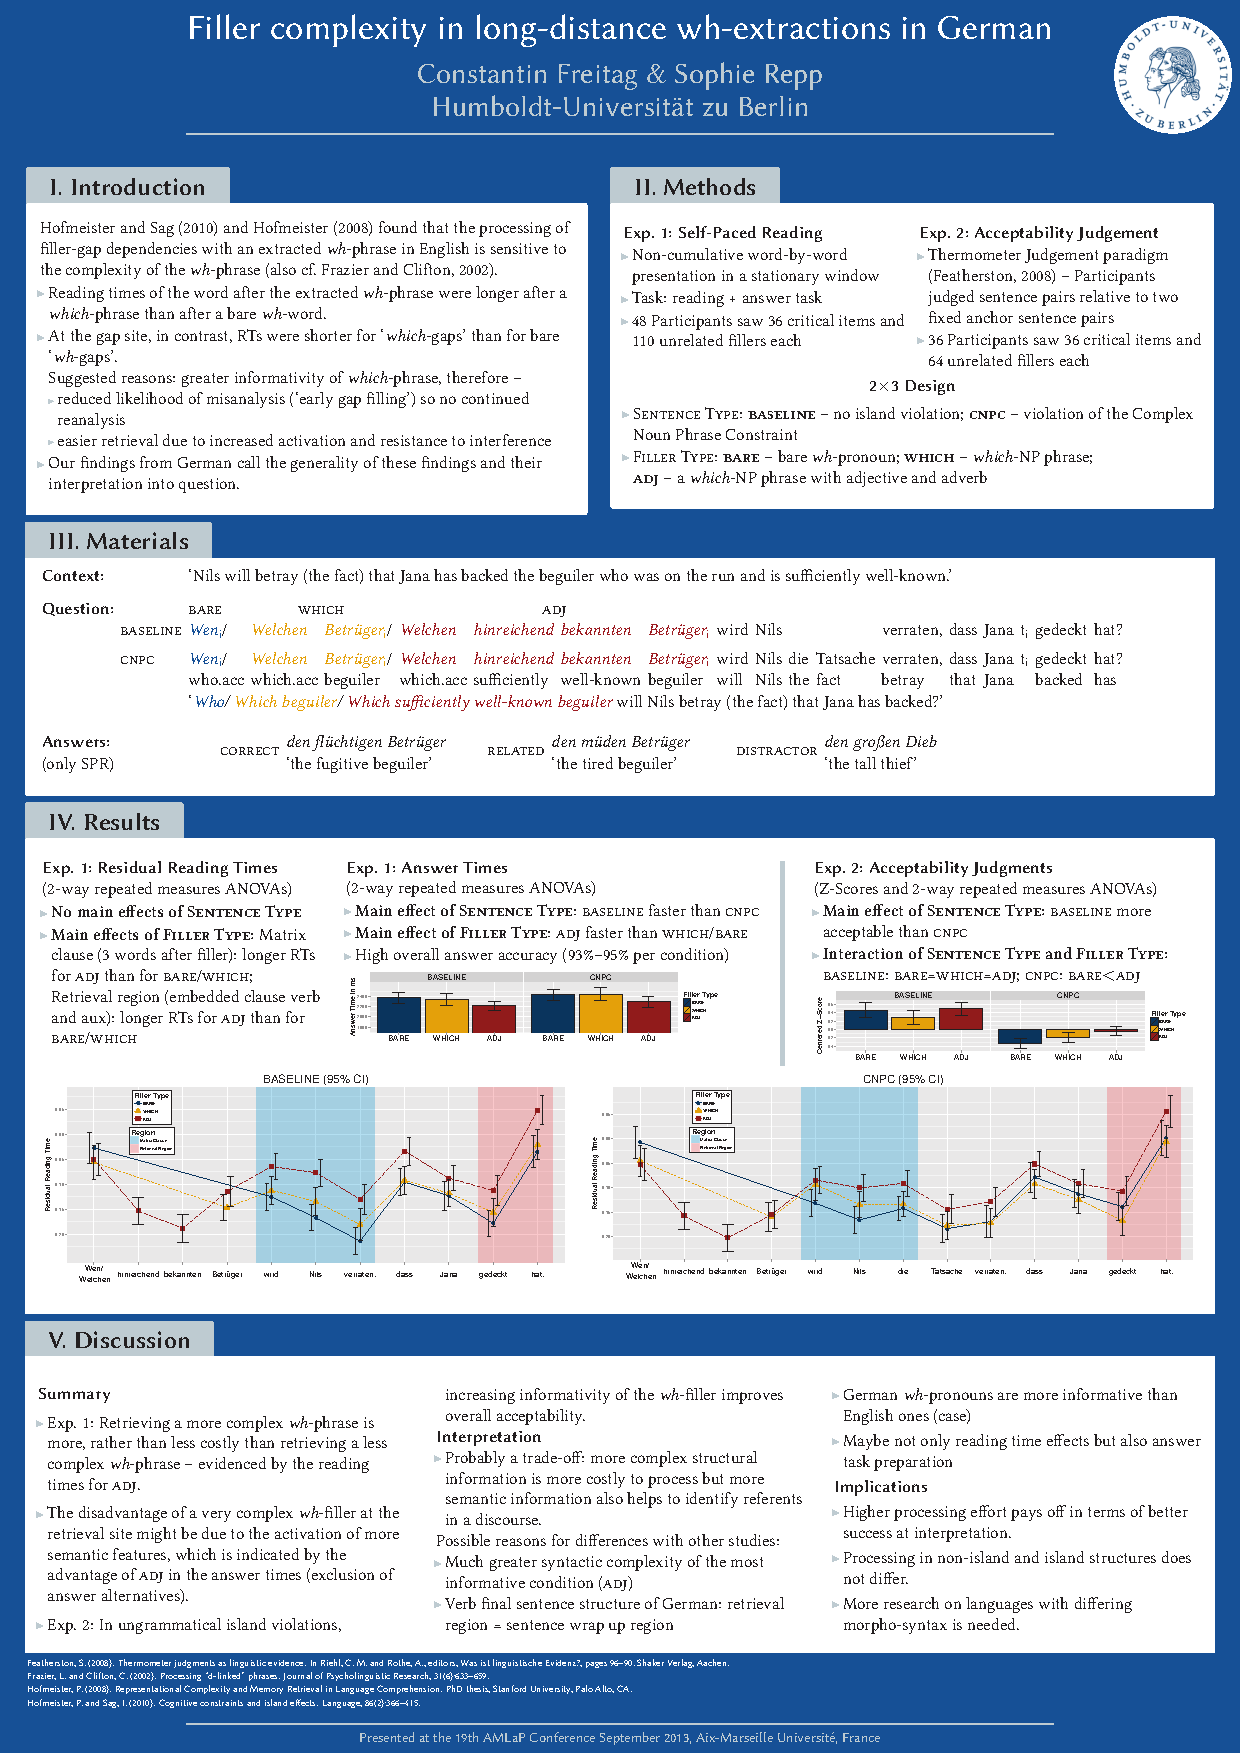
\includegraphics[width=0.80\linewidth]{../../texfiles-beamer/tex-material/WissArb-latex/Freitag_Repp_AMLaP_2013_A4.pdf}
\end{minipage}  
%  
\begin{minipage}[b]{0.49\textwidth}
\centering

\includegraphics[width=0.80\linewidth]{../../texfiles-beamer/tex-material/WissArb-latex/UKN_brief.pdf}
%\caption{Adjunkt und Komplement}	
\end{minipage}
%         
%\end{figure}

\end{frame}


%%%%%%%%%%%%%%%%%%%%%%%%%%%%%%%%%%%
\begin{frame}
\frametitle{Trees}

\begin{figure}

\begin{minipage}[b]{0.70\textwidth}
\centering
\footnotesize{
\begin{forest}
%sn edges,
[IP 
	[DP [Peter\\
	\emph{Peter},roof]]
	[\xprime{I} 
		[VP 
			[\xprime{V} 
				[DP [den Wagen\\
				\emph{the car}, roof]]
				[\xzero{V} [t$_{i}$,draw]{
				\draw[->,dotted] () to[out=south east,in=south] (IHead);}
				]
			]
		]
		[\xzero{I} 
			[\alert{kauft}$_{i}$\\
			\emph{buys},name=IHead]
		]{\draw[<-,red] (.south east)--++(0em,-1.5ex)--++(+2em,0pt)
node[anchor=west,align=center]{finite};}
	]
]
\end{forest}
}
\caption{Head movement}	
\end{minipage} 

\end{figure}

\end{frame}


%%%%%%%%%%%%%%%%%%%%%%%%%%%%%%%%%%%
\begin{frame}
\frametitle{Glossing \& IPA}

\ea 
	\ea
	\gll Der Mann schläf -t.\\
	the.\textsc{nom} man.\textsc{nom} sleep -s\\
	\glt `The man is sleeping.'

	\ex 
	%\settowidth\jamwidth{\textsc{Deutsch}}
	\gll Der Mann hat dem Jungen ein Buch über Linguistik gegeben.\\
	the.\textsc{nom} man.\textsc{nom} has the.\textsc{dat} boy.\textsc{dat} a.\textsc{acc} book.\textsc{acc} about linguistics give.\textsc{ptcp.prf}\\
	\glt `The man gave the boy a book about linguistics.' 
	%\jambox{\textsc{Deutsch}}
	\z 
		
\ex 
	\ea \ab{phonetics} 
	\ex {/}\textipa{f@".nE.tIks}/ 
	\ex {[}\textipa{f@"nEtIks}] 
	\z 
\z 

\end{frame}


%%%%%%%%%%%%%%%%%%%%%%%%%%%%%%%%%%%
%%%%%%%%%%%%%%%%%%%%%%%%%%%%%%%%%%%
\subsection{How does \LaTeX\ work?}
%\frame{
%	%\frametitle{~}
%	\begin{multicols}{2}
%		\tableofcontents[currentsection,hideallsubsections]
%	\end{multicols}
%}
%%%%%%%%%%%%%%%%%%%%%%%%%%%%%%%%%%%

\begin{frame}
\frametitle{How does \LaTeX\ work?}

By compiling your document, \LaTeX\ creates further \textbf{auxiliary files} to improve the next compilations.

\begin{columns}

\column[t]{.6\textwidth}

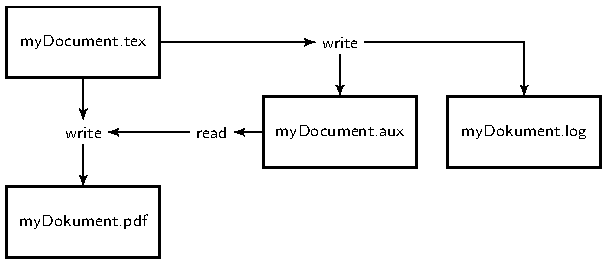
\includegraphics[scale=.75]{../../texfiles-beamer/tex-material/WissArb-latex/LaTeX-flowchart-1.pdf}

\column[t]{.4\textwidth}

\begin{itemize}
	\item your document: \ltxterm{.tex}
	\item your output: \ltxterm{.pdf}
\end{itemize}

\end{columns}

\end{frame}


%%%%%%%%%%%%%%%%%%%%%%%%%%%%%%%%%%%
\begin{frame}
%\frametitle{Wie funktioniert \LaTeX ?}

\begin{minipage}{.58\textwidth}

The auxiliary files can be \textbf{deleted} after your work is done. They will be created again when you compile.

\begin{itemize}
	\item \ltxterm{.log} \ras information about the compiling process
	
	\item \ltxterm{.bbl} \ras information for the bibliography
	
	\item \ltxterm{.nav} \ras information for the navigation through slides
	
	\item \ltxterm{.toc} \ras information for the table of contents
		
	\item \dots 
\end{itemize}

\end{minipage}
%
\begin{minipage}{.40\textwidth}
	\centering
	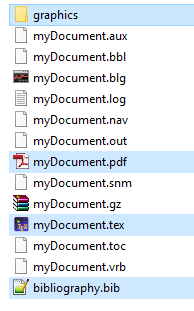
\includegraphics[width=.9\linewidth]{../../texfiles-beamer/tex-material/WissArb-latex/latexDateien}
	
\end{minipage}

\end{frame}


%%%%%%%%%%%%%%%%%%%%%%%%%%%%%%%%%%%
\begin{frame}
%\frametitle{Wie funktioniert \LaTeX ?}

\begin{minipage}{.58\textwidth}
	The following files are important and \textbf{should not be deleted}. They are not created in the compiling process:
		
	\begin{itemize}
		\item \texttt{.tex} \ras this is the document you are working on.
		
		\item \texttt{.pdf} \ras you can delete your PDF, but this is what you normally want as your result
		
		\item \texttt{.bib} \ras this file contains your bibliography data base (if you have one)
		
		\item folder \texttt{graphics} \ras here could be your graphics (if you need some)
	\end{itemize}
	
\end{minipage}
%
\begin{minipage}{.40\textwidth}
	\centering
	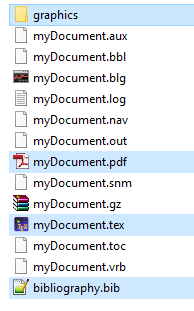
\includegraphics[width=.9\linewidth]{../../texfiles-beamer/tex-material/WissArb-latex/latexDateien}
	
\end{minipage}

\end{frame}

}
%% END handout true 
%% BEGIN handout false
{
%%%%%%%%%%%%%%%%%%%%%%%%%%%%%%%%%%

%% EMPTY

}%% END handout false
%%%%%%%%%%%%%%%%%%%%%%%%%%%%%%%%%%


%%%%%%%%%%%%%%%%%%%%%%%%%%%%%%%%%%%
%%%%%%%%%%%%%%%%%%%%%%%%%%%%%%%%%%%
\section{Overleaf}
%\frame{
%	%\frametitle{~}
%	\begin{multicols}{2}
%		\tableofcontents[currentsection,hideallsubsections]
%	\end{multicols}
%}
%%%%%%%%%%%%%%%%%%%%%%%%%%%%%%%%%%%

\begin{frame}
\frametitle{Overleaf}

\begin{enumerate}
	\item Go to: \url{https://www.overleaf.com}
	
	Overleaf is an online \LaTeX\ editor. 
	
	\item \textbf{Register} with your email address and create a new blank project.
	
	Your project is not completely empty. Overleaf provides already some information. Later, we are going to change this information.
	
	\item \textbf{Compile} your project: Click on the green button \emph{Recompile}.
	
	\item PDF\LaTeX\ is the \textbf{standard compiler}. 
	Write 5 > 4 after the section \emph{Introduction}, compile, and see what happens.
	
	\item \textbf{Change compiler}: Click on the Overleaf menu icon above the file list panel, and set the \emph{Compiler} setting to `Xe\LaTeX '.
	
	\item \textbf{Recompile} your project, and see what happens.
	
\end{enumerate}

\bigskip 

You will find the tasks for our course here: \url{https://github.com/langsci/latex4linguists/blob/master/1-1.md}

%In diesem Kurs werden wir mit dem \textbf{Editor} \texttt{TeXstudio} arbeiten, welcher folgende Vorteile anbietet: 
%
%\begin{itemize}
%	\item kostenlos, 
%	
%	\item kompatible mit Linux-, Windows- und Mac OS-Rechnern,
%	\item Unicode-Unterstützung, Rechtschreibkontrolle, Autovervollständigung von Befehlen, PDF-Viewer,
%	\item einfach zu verwenden und zu konfigurieren, \dots
%\end{itemize}
%
%Außer dem Editor benötigt man eine \LaTeX -\textbf{Distribution}.
%In diesem Fall werden wir \texttt{MiKTeX} (für Windows-User)
%verwenden. Für Linux-User ist \texttt{TeXLive} eine sehr bekannte Alternative und für Mac OS-User \texttt{MacTeX}. \textbf{Zuerst} soll die Distribution (\zB \texttt{MiKTeX}) und erst dann der Editor (\zB \texttt{TeXstudio}) installiert werden!

\end{frame}


%%%%%%%%%%%%%%%%%%%%%%%%%%%%%%%%%%


%%%%%%%%%%%%%%%%%%%%%%%%%%%%%%%%%%%%
%%%%%%%%%%%%%%%%%%%%%%%%%%%%%%%%%%%%
%\subsection{Software}
%%\frame{
%%	%\frametitle{~}
%%	\begin{multicols}{2}
%%		\tableofcontents[currentsection,hideallsubsections]
%%	\end{multicols}
%%}
%%%%%%%%%%%%%%%%%%%%%%%%%%%%%%%%%%%%
%
%\begin{frame}
%\frametitle{Software}
%
%In diesem Kurs werden wir mit dem \textbf{Editor} \texttt{TeXstudio} arbeiten, welcher folgende Vorteile anbietet: 
%
%\begin{itemize}
%	\item kostenlos, 
%	
%	\item kompatible mit Linux-, Windows- und Mac OS-Rechnern,
%	\item Unicode-Unterstützung, Rechtschreibkontrolle, Autovervollständigung von Befehlen, PDF-Viewer,
%	\item einfach zu verwenden und zu konfigurieren, \dots
%\end{itemize}
%
%Außer dem Editor benötigt man eine \LaTeX -\textbf{Distribution}.
%In diesem Fall werden wir \texttt{MiKTeX} (für Windows-User)
%verwenden. Für Linux-User ist \texttt{TeXLive} eine sehr bekannte Alternative und für Mac OS-User \texttt{MacTeX}. \textbf{Zuerst} soll die Distribution (\zB \texttt{MiKTeX}) und erst dann der Editor (\zB \texttt{TeXstudio}) installiert werden!
%
%\end{frame}


%%%%%%%%%%%%%%%%%%%%%%%%%%%%%%%%%%%
%%%%%%%%%%%%%%%%%%%%%%%%%%%%%%%%%%%
\section{Document structure 1}
\frame{
	%\frametitle{~}
	\begin{multicols}{2}
		\tableofcontents[currentsection,hideallsubsections]
	\end{multicols}
}
%%%%%%%%%%%%%%%%%%%%%%%%%%%%%%%%%%%


%%%%%%%%%%%%%%%%%%%%%%%%%%%%%%%%%%%%
%%%%%%%%%%%%%%%%%%%%%%%%%%%%%%%%%%%%
%\iftoggle{handout}{
%%% BEGIN handout true	
%%%%%%%%%%%%%%%%%%%%%%%%%%%%%%%%%%%%
	

%%%%%%%%%%%%%%%%%%%%%%%%%%%%%%%%%%%%
%\begin{frame}[fragile]
%\frametitle{Document structure 1}
%
%A \LaTeX document consists of (at least) two parts: \textbf{preamble} and \textbf{body}.
%
%\begin{block}{\LaTeX\ preamble}
%	part of the document where \textbf{global characteristics} of the document are specified.
%\end{block}
%
%\pause 
%
%	\begin{itemize}
%		\item The preamble \textbf{begins} (\textbf{obligatorily}) with the \lstinline|\documentclass{}| command.
%		
%		\item In the preamble you will install \textbf{packages} for further \LaTeX\ functions.
%		
%		\item \textbf{Optional} (either in the preamble or in the body -- preferably in the preamble)
%
%		\begin{itemize}
%			\item your \textbf{own commands} and 
%			
%			\item \textbf{metadata} 
%		\end{itemize}
%		
%		\item The preamble \textbf{ends} with the command  \lstinline|\begin{document}|.
%		
%	\end{itemize}
%
%\end{frame}


%%%%%%%%%%%%%%%%%%%%%%%%%%%%%%%%%%
%\begin{frame}[fragile]
%%\frametitle{Dokumentstruktur}
%
%
%\begin{block}{\LaTeX\ body}
%	part of the document where \textbf{local characteristics} of the document are specified and where you write your document.
%\end{block}
%
%\pause 
%
%\begin{itemize}
%	
%	\item The body \textbf{begins} with the \lstinline|\begin{document}| command  (end of preambel).
%	
%	\item The body \textbf{ends} with \lstinline|\end{document}|. 
%	
%	\item[]
%
%\pause 
%	
%	\item Everything following the command \lstinline|\end{document}| will not be interpreted by \LaTeX .
%\end{itemize}
%
%\end{frame}

%}
%%% END handout true 
%%% BEGIN handout false
%{
%%%%%%%%%%%%%%%%%%%%%%%%%%%%%%%%%%%


%%%%%%%%%%%%%%%%%%%%%%%%%%%%%%%%%
\begin{frame}
\frametitle{Document structure 1}

A \LaTeX\ document consists of (at least) two parts: \textbf{preamble} and \textbf{body}.

\begin{block}{\LaTeX\ preamble}
	part of the document where \textbf{global characteristics} of the document are specified.
\end{block}

\begin{block}{\LaTeX\ body}
	part of the document where \textbf{local characteristics} of the document are specified and where you write your document.
\end{block}

\end{frame}

%}%% END handout false
%%%%%%%%%%%%%%%%%%%%%%%%%%%%%%%%%%%


%%%%%%%%%%%%%%%%%%%%%%%%%%%%%%%%%
\begin{frame}[fragile]
\frametitle{Exercise}

\begin{itemize}
	\item Insert the following lines in your \ltxterm{.tex} file and compile.
\end{itemize}

\vspace{.25cm}

\centering
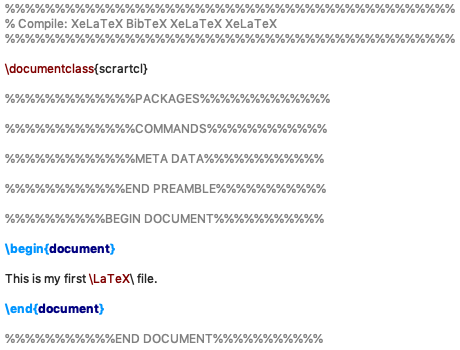
\includegraphics[scale=0.45]{../../texfiles-beamer/tex-material/WissArb-latex/xelatexTest1tex}

\begin{itemize}
	\item Write something after the \lstinline|\end{document}| command and compile again.	
\end{itemize}

\end{frame}


%%%%%%%%%%%%%%%%%%%%%%%%%%%%%%%%%%%%
%%%%%%%%%%%%%%%%%%%%%%%%%%%%%%%%%%%%
\section{Document class}
%\frame{
%	%\frametitle{~}
%	\begin{multicols}{2}
%		\tableofcontents[currentsection,hideallsubsections]
%	\end{multicols}
%}
%%%%%%%%%%%%%%%%%%%%%%%%%%%%%%%%%%%

\begin{frame}[fragile]
\frametitle{Document class}

Global parameters of the layout can be specified in the \lstinline|documentclass| command. The most commonly used classes are:
 
\begin{itemize}
	\item \ltxterm{book} for books
%	\item \ltxterm{report} for long scripts with different chapters
	\item \ltxterm{article} for articles, without chapters, only with sections
	\item \ltxterm{beamer} for presentations, without chapters, only with sections
%	\item \ltxterm{letter} for letters
\end{itemize}

\pause 

Variations of these classes (not in American formats) are provided by the \textbf{\ltxterm{KOMA-Script}}:

\begin{itemize}
	\item \ltxterm{scrbook} for books
%	\item \ltxterm{scrreprt} for long scripts with different chapters
	\item \alert{\ltxterm{scrartcl}} for articles, without chapters, only with sections
%	\item \ltxterm{scrlttr2} for letters
\end{itemize}

%Cf.\ \citet{Kohm&Co13a} and \url{https://www.komascript.de/}

\end{frame}


%%%%%%%%%%%%%%%%%%%%%%%%%%%%%%%%%%%%
\begin{frame}[fragile]

You can specify \textbf{options} in your \lstinline|documentclass| command.

\begin{itemize}
	\item \textbf{Font size} as default: \ltxterm{10pt}, \ltxterm{11pt}, \ltxterm{12pt} \par
	Default $\rightarrow$ \ltxterm{10pt} 
	
	\item \textbf{Paper format}: \ltxterm{letterpaper}, \ltxterm{a4paper} \par
	Default $\rightarrow$ \ltxterm{letterpaper}

\end{itemize}

Specification of paper format in \ltxterm{KOMA-Script} classes: \ltxterm{paper=a4},  \ltxterm{paper=letter}

\end{frame}


%%%%%%%%%%%%%%%%%%%%%%%%%%%%%%%%%
\begin{frame}[fragile]
\frametitle{Exercise}

\begin{itemize}
	\item Specify the following options for your document  \ltxterm{.tex} file and compile.
\end{itemize}

\vspace{.25cm}

\centering
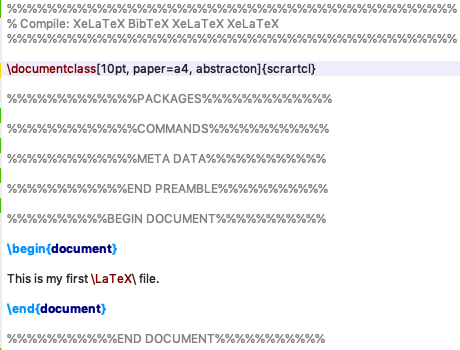
\includegraphics[scale=0.45]{../../texfiles-beamer/tex-material/WissArb-latex/xelatexTest2tex}

\end{frame}


%%%%%%%%%%%%%%%%%%%%%%%%%%%%%%%%%%%%
%\begin{frame}[fragile]
%\frametitle{Dokumentklasse}
%
%\begin{lstlisting}
%\documentclass[10pt,paper=a4]{scrartcl}
%\begin{document}
%Text Text Text
%\end{document}
%\end{lstlisting}
%
%\begin{description}
%\item[Hinweis:] \ltxterm{TeXstudio} bietet einen Assistenten, der die Präambel für Sie schreibt. Schauen Sie in der Toolbar unter \texttt{Assistenten/Assistent für ein neues Dokument} nach. Dort können Sie alles weitere einstellen.
%\end{description}
%
%\end{frame}


%%%%%%%%%%%%%%%%%%%%%%%%%%%%%%%%%%%
%%%%%%%%%%%%%%%%%%%%%%%%%%%%%%%%%%%
\section{Commands}
\frame{
	%\frametitle{~}
	\begin{multicols}{2}
		\tableofcontents[currentsection,hideallsubsections]
	\end{multicols}
}
%%%%%%%%%%%%%%%%%%%%%%%%%%%%%%%%%%%

%\begin{frame}[fragile]
%\frametitle{Commands}
%
%\textbf{Syntax of commands:}
%
%\begin{itemize}
%	
%	\item backslash \\
%	$+$ command name \\
%	$+$ optional arguments in square brackets \\
%	$+$ obligatory arguments in curly brackets
%
%\end{itemize}
%		
%\begin{lstlisting}
%\name[optional argument]{obligatory argument} 
%\name[opt1, opt2=value]{obl1}{obl2}
%
%\textbf{bold}
%\documentclass[10pt, paper=a4]{scrartcl}
%\end{lstlisting}
%
%\end{frame}


%%%%%%%%%%%%%%%%%%%%%%%%%%%%%%%%%%%
\begin{frame}[fragile]
\frametitle{Commands}

In \LaTeX , there are normally \textbf{3 types of commands}:

\begin{itemize}
	\item \textbf{declarations:} backslash $+$ command name\\
	The scope of the command can be defined by an environment or with curly brackets. 
\end{itemize}

\vspace{-.5cm}

\begin{columns}
	\column[t]{.5\textwidth}
	
\begin{lstlisting}
\declaration ... 
{\declaration ...} outside of scope

\end{lstlisting}
	
	\column[t]{.5\textwidth}	
	
\begin{lstlisting}
{\Huge Hello world!} outside of scope
\end{lstlisting}
	
\end{columns}

\pause

\begin{itemize}
	\item \textbf{simple commands:} backslash $+$ command name $+$ optional arguments (square brackets) $+$ obligatory arguments (curly brackets)
\end{itemize}

\vspace{-.5cm}

\begin{columns}
	\column[t]{.5\textwidth}
	
\begin{lstlisting}
\name[optional]{obligatory} 
\end{lstlisting}

	\column[t]{.5\textwidth}	
	
\begin{lstlisting}
\textit{Text in italics} 
\end{lstlisting}
	
\end{columns}

\pause 

\begin{itemize}
	\item \textbf{environments:} \ltxterm{begin} $+$ \ltxterm{end} command. \\
	Command applies between \ltxterm{begin} and \ltxterm{end}.
\end{itemize}

\vspace{-.5cm}

\begin{columns}
	\column[t]{.5\textwidth}
	
\begin{lstlisting}
\begin{environment}[optional]
...
\end{environment}

\end{lstlisting}

\column[t]{.5\textwidth}	

\begin{lstlisting}
\begin{center}
Hello world!
\end{center}
\end{lstlisting}

\end{columns}

\end{frame}


%%%%%%%%%%%%%%%%%%%%%%%%%%%%%%%%%%%
%%%%%%%%%%%%%%%%%%%%%%%%%%%%%%%%%%%
\section{Document structure 2}
\frame{
	%\frametitle{~}
	\begin{multicols}{2}
		\tableofcontents[currentsection,hideallsubsections]
	\end{multicols}
}
%%%%%%%%%%%%%%%%%%%%%%%%%%%%%%%%%%%

\begin{frame}[fragile]
\frametitle{Meta data}

Specifying the \textbf{meta data} of your document \textbf{in the preamble}: 

\begin{lstlisting}
\author{first name last name \and first name last name}
\title{my title}
\subtitle{my subtitle}
\date{14th Februar 2019}
\end{lstlisting}

\begin{itemize}
	\item Other options for date: \lstinline|\date{\today}|, \lstinline|\date{}|
	
	Default $\rightarrow$ \lstinline|\date{\today}|
\end{itemize}

Use the command \lstinline|\maketitle| after \lstinline|\begin{document}| to include this information in your output.
\end{frame}


%%%%%%%%%%%%%%%%%%%%%%%%%%%%%%%%%
\begin{frame}[fragile]
\frametitle{Exercise}

Specify the meta data in your document with two authors, use the  \lstinline|\maketitle| command, and try different commands for date.

\centering
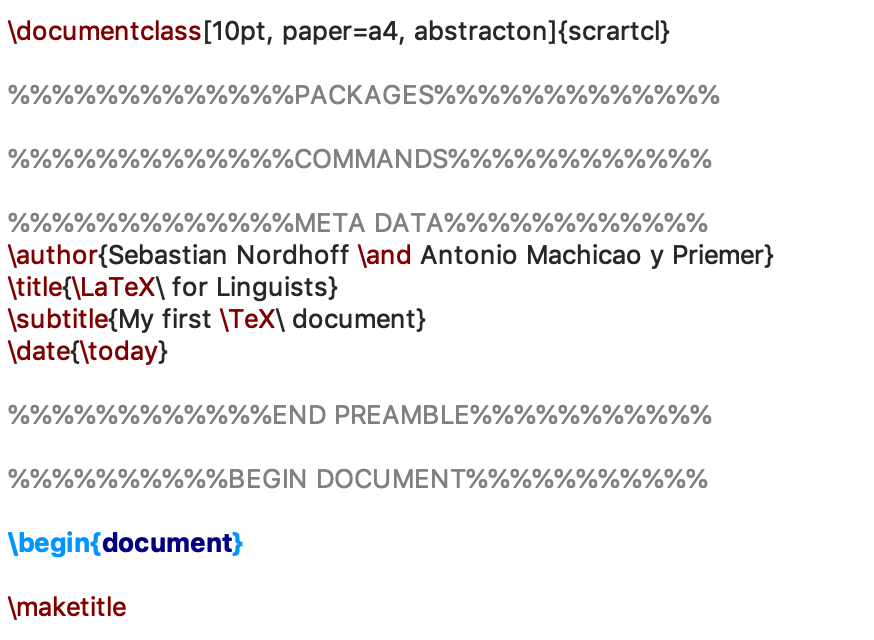
\includegraphics[width=0.65\linewidth]{../../texfiles-beamer/tex-material/WissArb-latex/xelatexTest3tex}

\end{frame}


%%%%%%%%%%%%%%%%%%%%%%%%%%%%%%%%%%%
%%%%%%%%%%%%%%%%%%%%%%%%%%%%%%%%%%%
\subsection{Headlines}
%\frame{
%	%\frametitle{~}
%	\begin{multicols}{2}
%		\tableofcontents[currentsection,hideallsubsections]
%	\end{multicols}
%}
%%%%%%%%%%%%%%%%%%%%%%%%%%%%%%%%%%%

\begin{frame}[fragile]
\frametitle{Headlines}

\noindent Commands for the structure of your text:

\begin{itemize}
	\item \lstinline|\part{title}|  \hfill (only in  \ltxterm{book}/\ltxterm{scrbook} and \ltxterm{report}/\ltxterm{scrreprt})
	
	\item \lstinline|\chapter{title}| \hfill (only in  \ltxterm{book}/\ltxterm{scrbook} and \ltxterm{report}/\ltxterm{scrreprt})
		
	\item \lstinline|\section{title}|
	
	\item \lstinline|\subsection{title}| 
	
	\item \lstinline|\subsubsection{title}| 
	
	\item \lstinline|\paragraph{title}|
	
	\item \lstinline|\subparagraph{title}|
\end{itemize}

\pause 

\bigskip

\noindent These commands can be used with an option, \fe\\

\lstinline|\section[short title]{long title}| 

\bigskip

The text in the \textbf{option} -- when used -- appears in the \textbf{table of contents} and in the \textbf{headers}, otherwise only the text in the \textbf{argument} is used.


\end{frame}


%%%%%%%%%%%%%%%%%%%%%%%%%%%%%%%%%%
%%%%%%%%%%%%%%%%%%%%%%%%%%%%%%%%%%
\subsection{Cross references 1}
%\label{sec:references}
%\frame{
%	\frametitle{~}
%	\begin{multicols}{2}
%		\tableofcontents[currentsection,hideallsubsections]
%	\end{multicols}
%}
%%%%%%%%%%%%%%%%%%%%%%%%%%%%%%%%%%

\begin{frame}[fragile]
\frametitle{Cross references 1}

To work with cross references, you need two things:

\begin{enumerate}
	\item a \ltxterm{label} with an \ltxterm{ID}: \lstinline|\label{ID}| 
	
	The \ltxterm{ID} must be \textbf{unique} for the labelled element in your document.
	
	\item a \ltxterm{reference}: \lstinline|\ref{ID}| 
	
	With the \lstinline|ref| command, \LaTeX\ will take the \textbf{number of element labelled} with the given \ltxterm{ID} and use it for cross references.
\end{enumerate}

\pause 

%\bigskip 

The \lstinline|label| command must \textbf{follow} (if possible: immediately) the element it is labelling.

%Wenn \LaTeX\ die \ltxterm{ID} des Eintrags \textbf{nicht findet}, weil man sich vielleicht verschrieben hat, wird statt des Verweises ein doppeltes Fragezeichen \ltxterm{??} stehen.

\bigskip 

The command \lstinline|\pageref{ID}| will give you the \textbf{page} in which the labelled element appears.

\begin{lstlisting}
\section{Introduction}
\label{sec:Intro}

To see how cross referencing works, take a look at Section \ref{sec:Intro} 
which is on page \pageref{sec:Intro}
\end{lstlisting}

\end{frame}


%%%%%%%%%%%%%%%%%%%%%%%%%%%%%%%%%%
\begin{frame}[fragile]
%\frametitle{Präfixe}

For long works, it is \textbf{useful} to have \textbf{prefixes}. They help you to find your references faster.

\begin{description}
\item[\ltxterm{sec}] for sections, subsections, \dots 
%\item[\ltxterm{ch}] nur für Kapitel 
%\item[\ltxterm{part}] nur für Bücher, die auch in Teile gegliedert sind (\ltxterm{sec} kann auch benutzt werden)
\item[\ltxterm{fig}] for figures
\item[\ltxterm{tab}] for tables
\item[\ltxterm{it}] for numbered items in lists
\item[\ltxterm{eq}] for equations
\item[\ltxterm{fn}] for footnotes
\end{description}


\begin{lstlisting}
\section{Introduction}
\label{sec:Intro}

To see how cross referencing works, take a look at Section \ref{sec:Intro} 
which is on page \pageref{sec:Intro}
\end{lstlisting}

\end{frame}


%%%%%%%%%%%%%%%%%%%%%%%%%%%%%%%%%%%
%%%%%%%%%%%%%%%%%%%%%%%%%%%%%%%%%%%
\subsection{Paragraphs \& line breaks}
%\frame{
%	%\frametitle{~}
%	\begin{multicols}{2}
%		\tableofcontents[currentsection,hideallsubsections]
%	\end{multicols}
%}
%%%%%%%%%%%%%%%%%%%%%%%%%%%%%%%%%%%

\begin{frame}[fragile]
\frametitle{Paragraphs \& line breaks}

\begin{itemize}
	\item new \textbf{paragraph}: twice \short{enter} (\rotatebox[origin=c]{180}{$\Rsh$}) key
%		\begin{itemize}
%			\item \lstinline|\par| ends a paragraph (and begins a new one)
%			\item twice \short{enter} (\rotatebox[origin=c]{180}{$\Rsh$}) key
%		\end{itemize}
	
	\item \textbf{line} break: \lstinline|\newline| or \lstinline|\\| cause a line break without ending the paragraph.
%		\begin{itemize}
%			\item \lstinline|\newline| or \lstinline|\\| cause a line break without ending the paragraph
%		\end{itemize}
	
	\item new \textbf{page}: \lstinline|\newpage| or \lstinline|\clearpage| 
	
	\item \lstinline|\noindent| \textbf{prevents} the \textbf{indentation} after a line break.
	
\end{itemize}

\end{frame}


%%%%%%%%%%%%%%%%%%%%%%%%%%%%%%%%%%%
%%%%%%%%%%%%%%%%%%%%%%%%%%%%%%%%%%%
\subsection{Table of contents}
%\frame{
%	%\frametitle{~}
%	\begin{multicols}{2}
%		\tableofcontents[currentsection,hideallsubsections]
%	\end{multicols}
%}
%%%%%%%%%%%%%%%%%%%%%%%%%%%%%%%%%%%

\begin{frame}[fragile]
\frametitle{Table of contents}

To \textbf{generate} a \textbf{table of contents} just include the following command in the body of your document at the position where you want the toc to appear.

\bigskip

\LaTeX\ generates your toc taking the \textbf{information from your structuring commands} (\fe \lstinline|\section[short title]{title}|).

\begin{lstlisting}
\tableofcontents
\end{lstlisting}

\end{frame}


%%%%%%%%%%%%%%%%%%%%%%%%%%%%%%%%%
\begin{frame}[fragile]
%\frametitle{Dokumentstruktur}

\centering
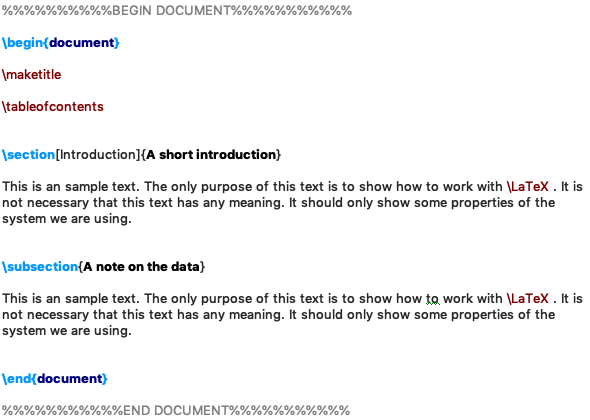
\includegraphics[width=0.84\linewidth]{../../texfiles-beamer/tex-material/WissArb-latex/xelatexTest4tex}


\end{frame}


%%%%%%%%%%%%%%%%%%%%%%%%%%%%%%%%%%%
%%%%%%%%%%%%%%%%%%%%%%%%%%%%%%%%%%%
\subsection{Footnotes}
%\frame{
%	%\frametitle{~}
%	\begin{multicols}{2}
%		\tableofcontents[currentsection,hideallsubsections]
%	\end{multicols}
%}
%%%%%%%%%%%%%%%%%%%%%%%%%%%%%%%%%%%

\begin{frame}[fragile]
\frametitle{Footnotes}

To generate a footnote use the following command at the position where the \textbf{footnote index} should appear. 

\begin{lstlisting}
\footnote{content of the footnote}
\end{lstlisting}

\noindent \textbf{Example}
\begin{lstlisting}
This is an sample text. The only purpose of this text\footnote{A text 
(literary theory) is any object that can be read.} is to show how 
to work with footnotes in \LaTeX .\footnote{\LaTeX\ is a document preparation 
system.}
\end{lstlisting}

%\pause 
%
%\noindent \textbf{Example 2}
%\begin{lstlisting}
%This is an sample text. The only purpose of this text%
%%
%\footnote{A text (literary theory) is any object that can be read.} %
%%
%is to show how to work with footnotes in \LaTeX .%
%%
%\footnote{\LaTeX\ is a document preparation system.}%
%%
%\end{lstlisting}

\end{frame}


%%%%%%%%%%%%%%%%%%%%%%%%%%%%%%%%%
\begin{frame}[fragile]
\frametitle{Exercise}

Go to \url{https://github.com/langsci/latex4linguists/blob/master/1-1.md}\\
and follow the instructions of the \textbf{first four blocks} in your \texttt{.tex} file.

\end{frame}


%%%%%%%%%%%%%%%%%%%%%%%%%%%%%%%%%%%
%%%%%%%%%%%%%%%%%%%%%%%%%%%%%%%%%%%
\section{Characters \& spaces}
\frame{
	%\frametitle{~}
	\begin{multicols}{2}
		\tableofcontents[currentsection,hideallsubsections]
	\end{multicols}
}
%%%%%%%%%%%%%%%%%%%%%%%%%%%%%%%%%%%


%%%%%%%%%%%%%%%%%%%%%%%%%%%%%%%%%%%
%%%%%%%%%%%%%%%%%%%%%%%%%%%%%%%%%%%
\subsection{Special characters}
%\frame{
%	%\frametitle{~}
%	\begin{multicols}{2}
%		\tableofcontents[currentsection,hideallsubsections]
%	\end{multicols}
%}
%%%%%%%%%%%%%%%%%%%%%%%%%%%%%%%%%%%

\begin{frame}[fragile]
\frametitle{Characters \& spaces}

\begin{itemize}
	
	\item The following characters can be used without problems:

\begin{lstlisting}
a...z  A...Z  0...9
. , : ; ? ! ` ' " ( ) + - * =
\end{lstlisting}

%\item Achten Sie darauf, welche Art von \textbf{Anführungszeichen} durch \lstinline|` ' "|  generiert werden \citep[vgl.][]{MyP17c}. 

%\item Die \textbf{Umlaute} \gqq{ä, ö, Ä, Ö, \dots}, \textbf{Akzente} \gqq{á, à, \dots} und das \textbf{Eszett} \gqq{ß} können (bei PDF-\LaTeX ) mithilfe des folgenden Pakets \lstinline|\usepackage[utf8]{inputenc}| direkt eingegeben werden.

\pause 

	\item With Xe\LaTeX , you can write \textbf{accents} and \textbf{umlauts} without further commands. Another option is to use \textbf{commands} for that:

\begin{lstlisting}
\"A \"O \"a \"o \'a \`o \ss{} \^u \~n

\"{A} {\"O} {\ss} 
\end{lstlisting}

	\ea \"A \"O \"a \"o \'a \`o \ss{} \^u \~n 
	
	\"{A} {\"O}  {\ss}
	\z 

\pause

	\item The following characters have a \textbf{special meaning} in \TeX . \\
	You must \textbf{escape} their function to use them. (It depends on your compiler \fe Xe\LaTeX\ \vs PDF\LaTeX )

\begin{lstlisting}
#  $  &  _  {  }  \  <  >  |  ~  ^  [  ]  % 
\end{lstlisting}

\end{itemize}

\end{frame}


%%%%%%%%%%%%%%%%%%%%%%%%%%%%%%%%%%%
\begin{frame}[fragile]
%\frametitle{Zeichen und Sonderzeichen}

\begin{itemize}
	
%		\item The following characters have a \textbf{special meaning} in \TeX . \\
%		You must \textbf{escape} their function to use them. (It depends on your compiler \fe Xe\LaTeX\ \vs PDF\LaTeX )
%	
%\begin{lstlisting}
%#  $  &  _  {  }  \  <  >  |  ~  ^  [  ]  % 
%\end{lstlisting}
%
%\pause

	\item escaping with \textbf{backslash} 

\begin{lstlisting}
\#  \$  \&  \_  \{  \}  \%
\end{lstlisting}
	
	\ea \#  \$  \&  \_  \{  \}  \%
	\z 
	
\pause 
	
	\item escaping with \textbf{macros} or \textbf{math mode}

\begin{lstlisting}
\textbackslash \textasciitilde \textasciicircum 
\textgreater $>$ \textless $<$ \textbar $\vert$  $|$  
\end{lstlisting}	
	\ea \textbackslash\ \textasciitilde\ \textasciicircum\ 
	\textgreater\ $>$ \textless\ $<$ \textbar\ $\vert$  $|$  
	\z 

\pause 
	
	\item \textbf{Angled brackets} < > can be used in Xe\LaTeX\ without further commands.
	
	\item \textbf{Square brackets} [ ] can be used in plain text, but they can mark also the \textbf{option} of a command (\fe in \lstinline|\section[short title]{title}|). \\
	In this case use \lstinline|\[ \]|
\end{itemize}

\bigskip 

More on special characters: \url{https://en.wikibooks.org/wiki/LaTeX/Special_Characters}
\end{frame}


%%%%%%%%%%%%%%%%%%%%%%%%%%%%%%%%%%%%
%\begin{frame}[fragile]
%%\frametitle{(Sonder-)Zeichen}
%
%\begin{itemize}
%
%	\item Dem \textbf{Backslash}, der \textbf{Größer-als}- und \textbf{Kleiner-als}-Zeichen, der \textbf{Tilde}, dem \textbf{Zirkumflex} und dem \textbf{senkrechten Strich} (\emph{pipe}) kann man nicht mit dem Backslash entkommen.
%
%\end{itemize}
%
%\end{frame}
%
%
%%%%%%%%%%%%%%%%%%%%%%%%%%%%%%%%%%%%
%\begin{frame}[fragile]
%%\frametitle{(Sonder-)Zeichen}
%
%\begin{itemize}
%
%\item Da die Folge \textbackslash\textbackslash\ für \textbf{Zeilenumbrüche} reserviert ist, kann man dem einfachen \textbf{Backslash} \gqq{\textbackslash} nicht mit Verwendung eines vorangestellten Backslashs entkommen. Dafür sollte der folgende Befehl benutzt werden:
%
%\begin{lstlisting}
%\textbackslash 
%\end{lstlisting}
%
%\item Die \textbf{Größer-als-} \gqq{\textgreater} und \textbf{Kleiner-als-Symbole} \gqq{\textless} können im Text durch die folgenden Befehle oder durch die Verwendung des Mathematikmodus', d.\,h. durch die \textbf{Klammerung in \$-Zeichen} erzeugt werden (mehr zum Mathematikmodus später).
%
%\begin{lstlisting}
%\textgreater $>$
%\textless $<$
%\end{lstlisting}
%
%\end{itemize}
%
%\end{frame}
%
%
%%%%%%%%%%%%%%%%%%%%%%%%%%%%%%%%%%%%
%\begin{frame}[fragile]
%%\frametitle{(Sonder-)Zeichen}
%
%\begin{itemize}
%
%\item Um den \textbf{senkrechten Strich} (\gq{pipe}) darzustellen, kann man entweder den Befehl \textbf{\texttt{vert}} oder den Strich in der \textbf{Mathematikmodusklammerung} eingeben oder den Befehl \textbf{\texttt{textbar}} außerhalb des Mathematikmodus'.
%
%\begin{lstlisting}
%$\vert$  $|$  \textbar
%\end{lstlisting}
%
%\item[]
%
%\item Die \textbf{Tilde} \gqq{\textasciitilde} hat in \LaTeX\ die Funktion eines geschützten Leerzeichens. Um dieser Funktion zu entkommen, kann man nicht den Backslash verwenden (\lstinline|\~|), denn dadurch erscheint der folgende Buchstabe mit einer Tilde. So bei der Eingabe \gqq{\texttt{\textbackslash\textasciitilde nicht}}, erscheint \gqq{\~nicht}. Will man auch dieser Funktion entkommen, muss der folgende Befehl (ähnlich wie bei dem Backslash) benutzt werden:
%
%\begin{lstlisting}
%\textasciitilde
%\end{lstlisting}
%
%\end{itemize}
%
%\end{frame}
%
%
%%%%%%%%%%%%%%%%%%%%%%%%%%%%%%%%%%%%%
%\begin{frame}[fragile]
%%\frametitle{(Sonder-)Zeichen}
%
%\begin{itemize}
%\item Das gleiche Problem taucht beim \textbf{Zirkumflex}  \gqq{\textasciicircum} auf, welcher als Akzent \zB im Französischen gebraucht wird. Daher erscheint bei der Eingabe \gqq{\texttt{s\textbackslash\textasciicircum ur}} der folgende Output: \gqq{s\^ur}. Aus diesem Grund benötigt man den folgenden Befehl um den Zirkumflex als Output zu haben:
%
%\begin{lstlisting}
%\textasciicircum
%\end{lstlisting}
%
%\item[]
%
%\item Weiteres zu Sonderzeichen in \LaTeX :
%
%\url{https://de.wikibooks.org/wiki/LaTeX/_Akzente_und_Sonderzeichen}
%
%\end{itemize}
%
%\end{frame}


%%%%%%%%%%%%%%%%%%%%%%%%%%%%%%%%%%
%%%%%%%%%%%%%%%%%%%%%%%%%%%%%%%%%%
\subsection{Space \& line break}
%\frame{
%	%\frametitle{~}
%	\begin{multicols}{2}
%		\tableofcontents[currentsection,hideallsubsections]
%	\end{multicols}
%}
%%%%%%%%%%%%%%%%%%%%%%%%%%%%%%%%%%

\begin{frame}
\frametitle{Space \& line break}

special treatment of \textbf{spaces} and \textbf{line breaks} to avoid typographic errors

\begin{itemize}

\item \textbf{no difference} between a \textbf{blank} and a \textbf{tab}

\item \textbf{Consecutive blanks} are treated as only one blank.

\item A \textbf{blank} at the \textbf{beginning of a line} is ignored.

\item One \textbf{line break} (1x \short{enter}) is interpreted as a blank.

\item One \textbf{empty line} (2x \short{enter}) is interpreted as the end of a paragraph.

\item \textbf{More than one empty line} is interpreted as one empty line.

\end{itemize}

\end{frame}


%%%%%%%%%%%%%%%%%%%%%%%%%%%%%%%%%%%
\begin{frame}[fragile]
%\frametitle{Leerzeichen}

\textbf{Example}

\begin{lstlisting}
   This is        a sample             text with too    many spaces. Here, I use one 
line break.
This is a sample text. Now, I use one blank line.

This is a sample text. Now, I use 3 blank lines.



This is a sample text. 
\end{lstlisting}

\pause 

\outputbox{
   This is        a sample             text with too    many spaces. Here, I use one 
line break.
This is a sample text. Now, I use one blank line.

This is a sample text. Now, I use 3 blank lines.



This is a sample text. 
}

\end{frame}


%%%%%%%%%%%%%%%%%%%%%%%%%%%%%%%%%%%
%%%%%%%%%%%%%%%%%%%%%%%%%%%%%%%%%%%
\section{Commenting out}
\frame{
	%\frametitle{~}
	\begin{multicols}{2}
		\tableofcontents[currentsection,hideallsubsections]
	\end{multicols}
}
%%%%%%%%%%%%%%%%%%%%%%%%%%%%%%%%%%%

\begin{frame}[fragile]
\frametitle{Commenting out}

In \LaTeX , text following the character \textbf{\%} in a line will be \textbf{ignored}.

\begin{itemize}
\item \textbf{hiding code/text}, without deleting it;

\item \textbf{finding errors} in sections;

\item \textbf{avoiding blanks} and \textbf{empty lines} in a long input line;

\item \textbf{writing comments} without seeing it in the output.

\end{itemize}

\begin{lstlisting}
This is a sample text. %This are just notes
%Here is a special characters and a command: & \small

A comment can divide a word:
Rindfleischetikettierungs% 5 morphemes
überwachungsaufgaben% 6 morphemes
übertragungsgesetz. 
\end{lstlisting}

\outputbox{
This is a sample text. %This are just notes
%Here is a special characters and a command: & \small

A comment can divide a word:
Rindfleischetikettierungs% 5 morphemes
überwachungsaufgaben-% 6 morphemes
übertragungsgesetz. 
}

\end{frame}


%%%%%%%%%%%%%%%%%%%%%%%%%%%%%%%%%%%
%%%%%%%%%%%%%%%%%%%%%%%%%%%%%%%%%%%
\section{Text formatting}
\frame{
	%\frametitle{~}
	\begin{multicols}{2}
		\tableofcontents[currentsection,hideallsubsections]
	\end{multicols}
}
%%%%%%%%%%%%%%%%%%%%%%%%%%%%%%%%%%%

\begin{frame}[fragile]
\frametitle{Text formatting}

%\LaTeX\ bietet verschiedene Befehle zur Textauszeichnung:

\begin{multicols}{2}
	
\begin{lstlisting}
\textbf{bold} 
\textit{italics}
\textsl{slanted} 
\emph{emphasized} 
{\it test \textup{upright} test}
\texttt{typewriter} 
\textsc{small caps} 
ex\textsuperscript{up} 
ex\textsubscript{down} 
\end{lstlisting}
	
\outputbox{
	\textbf{bold}\newline 
	\textit{italics}\newline
	\textsl{slanted}\newline 
	\emph{emphasized}\newline 
	{\it test \textup{upright} test}\newline 
%	\underline{underline}\newline 
	\texttt{typewriter}\newline
	\textsc{small caps}\newline 
	ex\textsuperscript{up} \newline
	ex\textsubscript{down} %\newline
}
	
\end{multicols}

Some of these commands can be also used as \textbf{declarations}. 
\end{frame}


%%%%%%%%%%%%%%%%%%%%%%%%%%%%%%%%%%%
\begin{frame}[fragile]
%\frametitle{Textauszeichnung}

%\LaTeX\ bietet auch die Möglichkeit an, die Schriftgröße zu ändern. Dies ist jedoch in wissenschaftlichen Arbeiten nicht empfehlenswert. Die Schriftgrößenbefehle können entweder als \textbf{Deklarationen} wie auch als \textbf{Umgebungen} angegeben werden.

\begin{multicols}{2}
\begin{lstlisting}
{\tiny tiny} 
{\scriptsize scsize} 
{\footnotesize fnsize} 
{\small small} 
{\normalsize normal} 
{\large large} 
{\Large Large} 
{\LARGE LARGE} 
{\huge huge} 
{\Huge Huge} 
\end{lstlisting} 
\columnbreak{}
\outputbox{
	{\tiny{tiny}\newline 
		\scriptsize{scsize}\newline
		\footnotesize{fnsize}\newline
		\small{small}\newline
		\normalsize{normal}\newline
		\large{large}\newline
		\Large{Large}\newline  
		\LARGE{LARGE}\newline
		\huge{huge}\newline
		\Huge{Huge}}
}
\end{multicols}

The commands for font size can be used as \textbf{declarations} or as \textbf{environments}.
\end{frame}


%%%%%%%%%%%%%%%%%%%%%%%%%%%%%%%%%
\begin{frame}[fragile]
\frametitle{Exercise}


Go to \url{https://github.com/langsci/latex4linguists/blob/master/1-1.md}\\
and follow the instructions of the \textbf{fifth block} in your \texttt{.tex} file.

\bigskip 

Test further commands!

%Download the PDF \alert{\texttt{myDocument-EX2.pdf}} and replicate it with the commands you have already learnt.

\end{frame}


%%%%%%%%%%%%%%%%%%%%%%%%%%%%%%%%%%%
%%%%%%%%%%%%%%%%%%%%%%%%%%%%%%%%%%%
\section{Text environments}
\frame{
	%\frametitle{~}
	\begin{multicols}{2}
		\tableofcontents[currentsection,hideallsubsections]
	\end{multicols}
}

%%%%%%%%%%%%%%%%%%%%%%%%%%%%%%%%%

\begin{frame}[fragile]
\frametitle{Text environments}
You will normally need the following text environments:

\begin{itemize}
	\item quotations,
	
	\item lists, 
	
%	\item \gqq{wörtliche Wiedergaben} und 
	
	\item abstracts,
	
%	\item examples (\dots\ later),
	
	\item \dots 
\end{itemize}

\end{frame}


%%%%%%%%%%%%%%%%%%%%%%%%%%%%%%%%%%%
%%%%%%%%%%%%%%%%%%%%%%%%%%%%%%%%%%%
\subsection{Quotations}
%\frame{
%	%\frametitle{~}
%	\begin{multicols}{2}
%		\tableofcontents[currentsection,hideallsubsections]
%	\end{multicols}
%}
%%%%%%%%%%%%%%%%%%%%%%%%%%%%%%%%%%%

\begin{frame}[fragile]
\frametitle{Quotations}
\begin{itemize}
	
%\item Wörtliche Zitate, die länger als zwei Zeilen lang sind, sollen \textbf{vom Fließtext getrennt} werden.

\item In \LaTeX\, there are two environments for quotations \ltxterm{quote} and \ltxterm{quotation}.

\item Both show a different output dependent on the document class (\fe \ltxterm{beamer} \vs \ltxterm{article}).

%\item Der Unterschied zwischen den beiden Befehlen betrifft die \textbf{Absatzgrenzen}.

%\begin{itemize}
%	\item \ltxterm{quote} trennt die Absätze mit vertikalem Abstand, 
%	
%	\item während \ltxterm{quotation} die erste Zeile jedes Absatzes einrückt.		
%\end{itemize}
%
%\item In der \ltxterm{beamer}-Klasse werden Zitate zusätzlich kursiviert.
\end{itemize}
%\end{frame}
%
%
%%%%%%%%%%%%%%%%%%%%%%%%%%%%%%%%%%%%
%\begin{frame}[fragile]
%\frametitle{Quote-Umgebung}


\begin{lstlisting}
This is a sentence before the \texttt{quote} environment.
\begin{quote}
Furthermore, each actual ``language'' will incorporate a periphery of borrowings,
historical residues, inventions, and so on, which we can hardly expect to -- and
indeed would not want to -- incorporate within a principled theory of UG. [\dots]

Viewed against the reality of what a particular person may have inside
his head, core grammar is an idealization.
\hfill (Chomsky,~1981:~8)
\end{quote}
This is a sentence after the \texttt{quote} environment.
\end{lstlisting}

%\end{frame}
%
%
%%%%%%%%%%%%%%%%%%%%%%%%%%%%%%%%%%%%
%\begin{frame}[fragile]
%\frametitle{Quote-Umgebung}

%\outputbox{
%This is a sentence before the \texttt{quote} environment.
%\begin{quote}
%	Furthermore, each actual ``language'' will incorporate a periphery of borrowings,
%	historical residues, inventions, and so on, which we can hardly expect to -- and
%	indeed would not want to -- incorporate within a principled theory of UG. [\dots]
%	
%	Viewed against the reality of what a particular person may have inside
%	his head, core grammar is an idealization.
%	\hfill (Chomsky,~1981:~8)
%\end{quote}
%This is a sentence after the \texttt{quote} environment.
%}
%
%%\nocite{Nolda&Co14a}

\nocite{Chomsky81b}

\end{frame}


%%%%%%%%%%%%%%%%%%%%%%%%%%%%%%%%%%%%
%\begin{frame}[fragile]
%\frametitle{Quotation-Umgebung}
%
%
%\begin{lstlisting}
%Das ist der Text vor der \texttt{quotation}-Umgebung.
%
%\begin{quotation}
%Die grammatischen Phänomene in einer Sprache 
%zerfallen in zwei Teilbereiche: kerngrammatische und 
%randgrammatische Phänomene (\emph{Ausnahmen}).
%\end{quotation}
%Das ist der Text nach der \texttt{quotation}-Umgebung.
%\end{lstlisting}
%
%\outputbox{
%Das ist der Text vor der \texttt{quotation}-Umgebung.
%
%\begin{quotation}
%Die grammatischen Phänomene in einer Sprache 
%zerfallen in zwei Teilbereiche: kerngrammatische und 
%randgrammatische Phänomene (\emph{Ausnahmen}).
%\end{quotation}
%Das ist der Text nach der \texttt{quotation}-Umgebung.
%}
%
%\nocite{Nolda&Co14a}
%
%\end{frame}


%%%%%%%%%%%%%%%%%%%%%%%%%%%%%%%%%%%
%%%%%%%%%%%%%%%%%%%%%%%%%%%%%%%%%%%
\subsection{List environments}
%\frame{
%	%\frametitle{~}
%	\begin{multicols}{2}
%		\tableofcontents[currentsection,hideallsubsections]
%	\end{multicols}
%}
%%%%%%%%%%%%%%%%%%%%%%%%%%%%%%%%%%%

\begin{frame}[fragile]
\frametitle{List environments}

\LaTeX\ has 3 pre-defined and 1 general list environments:

\begin{itemize}
	\item \alert<2->{\ltxterm{itemize}},
	\item \alert<2->{\ltxterm{enumerate}},
	\item \alert<2->{\ltxterm{description}},

	\item \ltxterm{list}.
\end{itemize}

\pause 

Every environment begins with the \lstinline|\begin{ }| and ends with the \lstinline|\end{ }| command.

Each point in the list begins with \lstinline|\item|.  
%\end{frame}
%
%%%%%%%%%%%%%%%%%%%%%%%%%%%%%%%%%%%%
%\begin{frame}[fragile]
%\frametitle{Itemize}
%
%Die \ltxterm{itemize}-Umgebung wird für ungeordnete Listen verwendet. 

\begin{multicols}{2}
\begin{lstlisting}
\begin{itemize}
\item syntax
\item semantics 

\begin{itemize}
\item lexical semantics
\item propositional semantics
\end{itemize}

\item morphology
\end{itemize}
\end{lstlisting}
\columnbreak{}
\outputbox{
\begin{itemize}
	\item syntax
	\item semantics 
	
	\begin{itemize}
		\item lexical semantics
		\item propositional semantics
	\end{itemize}
	
	\item morphology
\end{itemize}
}
\end{multicols}

\end{frame}

%%%%%%%%%%%%%%%%%%%%%%%%%%%%%%%%%%%%
%\begin{frame}[fragile]
%\frametitle{Enumerate}
%
%Nummerierte Listen werden mit der \ltxterm{enumerate}-Umgebung erzielt.
%
%\begin{multicols}{2}
%
%\begin{lstlisting}
%\begin{enumerate}
%\item erster Punkt
%\item zweiter Punkt
%
%\begin{enumerate}
%\item Unterpunkt 1
%\item Unterpunkt 2
%\end{enumerate}
%
%\item dritter Punkt
%\end{enumerate}
%\end{lstlisting}
%\columnbreak{}
%\outputbox{
%\begin{enumerate}
%\item erster Punkt
%\item zweiter Punkt
%
%\begin{enumerate}
%\item Unterpunkt 1
%\item Unterpunkt 2
%\end{enumerate}
%
%\item dritter Punkt
%\end{enumerate}
%}
%\end{multicols}
%
%\end{frame}

%%%%%%%%%%%%%%%%%%%%%%%%%%%%%%%%%%%
\begin{frame}[fragile]
%\frametitle{Description}

The \ltxterm{description} list can be used for terms with their definitions.

\begin{lstlisting}
\begin{description}
\item[Morpheme:] smallest grammatical unit in a language bearing a meaning

\begin{description}
\item[Allomorph:] phonetic variant of a morpheme 
\end{description}

\item[Phoneme:] systematic unit of sound (or gesture in the case of sign 
languages, see chereme) that distinguish one word from another in a particular 
language
\end{description}
\end{lstlisting}

%\end{frame}
%
%
%%%%%%%%%%%%%%%%%%%%%%%%%%%%%%%%%%%%
%\begin{frame}[fragile]
%%\frametitle{Description}

\outputbox{
\begin{description}
	\item[Morpheme:] smallest grammatical unit in a language bearing a meaning
	
	\begin{description}
		\item[Allomorph:] phonetic variant of a morpheme 
	\end{description}
	
	\item[Phoneme:] systematic unit of sound (or gesture in the case of sign 
	languages, see chereme) that distinguish one word from another in a particular 
	language
\end{description}
}


% MyP: Welchen Unterschied?
%\vspace{\baselineskip}
%\noindent Bitte beachten Sie den Unterschied zwischen den Befehlen \textbackslash\textbackslash\ und \lstinline|\par|.
\end{frame}


%%%%%%%%%%%%%%%%%%%%%%%%%%%%%%%%%%%
\begin{frame}[fragile]
\frametitle{Combining lists}

Lists can be \textbf{combined} and \textbf{embedded} in other list types. 

\begin{multicols}{2}
\begin{lstlisting}
\begin{description}
\item[Morpheme:] smallest grammatical 
unit in a language bearing a meaning

\begin{itemize}
\item minimal unit in morphology
\item subtypes:

\begin{enumerate}
\item roots
\item prefixes
\item suffixes
\item \dots
\end{enumerate}

\end{itemize}

\end{description}
\end{lstlisting}
\columnbreak{}
\outputbox{
\begin{description}
	\item[Morpheme:] smallest grammatical 
	unit in a language bearing a meaning
	
	\begin{itemize}
		\item minimal unit in morphology
		\item subtypes:
		
		\begin{enumerate}
			\item roots
			\item prefixes
			\item suffixes
			\item \dots
		\end{enumerate}
		
	\end{itemize}
	
\end{description}
}
\end{multicols}
\end{frame}


%%%%%%%%%%%%%%%%%%%%%%%%%%%%%%%%%%%
\begin{frame}[fragile]
\frametitle{Customizing lists}

\noindent Bullet points can be customized with an \textbf{optional parameter}.

\begin{multicols}{2}

\begin{lstlisting}
\begin{itemize}
\item standard symbol
\item[+] customized
\item[--] customized
\item[--] customized
\end{itemize}
\end{lstlisting}

\columnbreak{}

\outputbox{
\begin{itemize}
	\item standard symbol
	\item[+] customized
	\item[--] customized
	\item[--] customized
\end{itemize}
}
\end{multicols}

\begin{multicols}{2}

\begin{lstlisting}
\begin{enumerate}
\item standard symbol
\item[+] customized
\item[+] customized
\item[--] customized
\item standard symbol
\end{enumerate}
\end{lstlisting}

\columnbreak{}

\outputbox{
\begin{enumerate}
	\item standard symbol
	\item[+] customized
	\item[+] customized
	\item[--] customized
	\item standard symbol
\end{enumerate}
}

\end{multicols}

\end{frame}


%%%%%%%%%%%%%%%%%%%%%%%%%%%%%%%%%%%
%%%%%%%%%%%%%%%%%%%%%%%%%%%%%%%%%%%
\subsection{Abstract}
%\frame{
%	%\frametitle{~}
%	\begin{multicols}{2}
%		\tableofcontents[currentsection,hideallsubsections]
%	\end{multicols}
%}
%%%%%%%%%%%%%%%%%%%%%%%%%%%%%%%%%%%

\begin{frame}[fragile]
\frametitle{Abstract}

For automatic abstracts, use the option \ltxterm{abstracton} in the \lstinline|\documentclass| command.

{\small
\begin{lstlisting}
\begin{abstract}
An abstract is a brief summary of a research article, thesis, or any in-depth 
analysis of a particular subject and is often used to help the reader quickly 
ascertain the paper's purpose.\par 
When used, an abstract always appears at the beginning of a manuscript, acting 
as the point-of-entry for any given academic paper. 
\end{abstract}
\end{lstlisting}
}
\outputbox{
\begin{abstract}
An abstract is a brief summary of a research article, thesis, or any in-depth 
analysis of a particular subject and is often used to help the reader quickly 
ascertain the paper's purpose.\par 
When used, an abstract always appears at the beginning of a manuscript, acting 
as the point-of-entry for any given academic paper. 
\end{abstract}
}

\end{frame}


%%%%%%%%%%%%%%%%%%%%%%%%%%%%%%%%%
\begin{frame}[fragile]
\frametitle{Exercise}


Go to \url{https://github.com/langsci/latex4linguists/blob/master/1-1.md}\\
and follow the instructions of the \textbf{blocks 6--8} in your \texttt{.tex} file.

\bigskip 

Test further commands!


%Download the PDF \alert{\texttt{myDocument-EX3.pdf}} and replicate it with the commands you have already learnt.

\end{frame}


%%%%%%%%%%%%%%%%%%%%%%%%%%%%%%%%%%%
%%%%%%%%%%%%%%%%%%%%%%%%%%%%%%%%%%%
\section{Loading packages}
\frame{
	%\frametitle{~}
	\begin{multicols}{2}
		\tableofcontents[currentsection,hideallsubsections]
	\end{multicols}
}

%%%%%%%%%%%%%%%%%%%%%%%%%%%%%%%%%

\begin{frame}[fragile]
\frametitle{Loading Packages}

\begin{itemize}
	\item The functions \LaTeX\ offers are restricted. Most \textbf{extra features} you will need are in \textbf{packages} that you can load in your \TeX\ document.

	\item Packages must be loaded in the \textbf{preamble} of your document.
\end{itemize}

\begin{lstlisting}
\usepackage[parameter1, parameter2]{package name}
\end{lstlisting}

\pause 

\begin{itemize}
\item Normally, (many) \LaTeX\ packages are already  \textbf{pre-installed} in your \TeX\ distribution (\fe \href{http://miktex.org/}{\ltxterm{MiKTeX}}).

\item (Almost) every other package (and its manual) can be \textbf{downloaded} from \textbf{\ltxterm{CTAN}} -- The Comprehensive \TeX\ Archive Network (\url{http://www.ctan.org/})
%(\href{http://www.ctan.org/}{www.ctan.org})

\item With the command \lstinline|usepackage| your \TeX\ distribution loads the package\\
 -- or  \textbf{downloads it automatically} if necessary.

\end{itemize}
\end{frame}


%%%%%%%%%%%%%%%%%%%%%%%%%%%%%%%%%%%
\begin{frame}[fragile]
%\frametitle{Pakete einbinden}

These packages can be useful:
\begin{itemize}

%\item Kodierung (Input): \ltxterm{inputenc}
%\lstinline|\usepackage[utf8]{inputenc}|

\item Language package: \ltxterm{babel} \hfill 
\lstinline|\usepackage[ngerman, english]{babel}|

%\item Kodierung (Font): \ltxterm{fontenc}
%\lstinline|\usepackage[T1]{fontenc}|

\item Font: \ltxterm{libertine} \hfill 
\lstinline|\usepackage{libertine}|

\item Blind text: \ltxterm{blindtext} \hfill 
\lstinline|\usepackage{blindtext}|

\item URLs: \ltxterm{url} \hfill 
\lstinline|\usepackage{url}|

\item Links (\fe for cross references): \ltxterm{hyperref} \\
\hfill 
\lstinline|\usepackage[bookmarksnumbered, hidelinks]{hyperref}|
\end{itemize}

Sometimes the \textbf{order} in that packages have been installed can affect the compilation (\fe \ltxpack{gb4e} and \ltxpack{forest}).

\bigskip 

Also, not all packages are \textbf{compatible} with each other or with your compiler (Xe\TeX\ \vs PDF\LaTeX ).

\end{frame}


%%%%%%%%%%%%%%%%%%%%%%%%%%%%%%%%%
\begin{frame}[fragile]
\frametitle{Exercise}


Go to \url{https://github.com/langsci/latex4linguists/blob/master/1-1.md}\\
and follow the instructions of the \textbf{blocks 9--11} in your \texttt{.tex} file.

\bigskip 

Test further commands!

%Download the PDF \alert{\texttt{myDocument-EX4.pdf}} and replicate it with the commands you have already learnt. Follow the instructions in the last section and install the packages.

\end{frame}


%%%%%%%%%%%%%%%%%%%%%%%%%%%%%%%%%%%
%%%%%%%%%%%%%%%%%%%%%%%%%%%%%%%%%%%
%\section{XY}
%%\frame{
%%\begin{multicols}{2}
%%\frametitle{~}
%%	\tableofcontents[currentsection]
%%\end{multicols}
%%}
%%%%%%%%%%%%%%%%%%%%%%%%%%%%%%%%%%%
%
%\begin{frame}{XY}
%
%\begin{itemize}
%	\item XY
%\end{itemize}
%
%\end{frame}


%%%%%%%%%%%%%%%%%%%%%%%%%%%%%%%%%%%%
%%%%%%%%%%%%%%%%%%%%%%%%%%%%%%%%%%%%
%\iftoggle{handout}{
%%% BEGIN handout true
%	
%%% EMPTY
%
%}
%%% END handout true 
%%% BEGIN handout false
%{
%%%%%%%%%%%%%%%%%%%%%%%%%%%%%%%%%%%%
%
%%% EMPTY
%
%}%% END handout false
%%%%%%%%%%%%%%%%%%%%%%%%%%%%%%%%%%%%